% REMEMBER: You must not plagiarise anything in your report. Be extremely careful.

\documentclass{l4proj}

    
% put any additional packages here
\usepackage{amsthm}
\usepackage{amssymb}
\usepackage{amsmath}
\usepackage{enumitem}
\usepackage{subcaption}

%==============================================================================
%% Commands 
\theoremstyle{definition}
\newtheorem{definition}{Definition}[section]

\newtheorem{proposition}{Proposition}[section]
\newtheorem{example}{Example}[section]

\DeclareMathAlphabet{\mathcal}{OMS}{cmsy}{m}{n}

\newcommand{\codefont}[1]{{\fontfamily{qcr}\selectfont #1}}

\setitemize{noitemsep}
%==============================================================================

\begin{document}

%==============================================================================
%% METADATA
\title{An Analysis on the Robustness of Watermarking Generative Text}
\author{Samuel Jackson}
\date{\today}

\maketitle

%==============================================================================
%% ABSTRACT
\begin{abstract}
    \textbf{Every abstract follows a similar pattern. Motivate; set aims; describe work; explain results.}
    \vskip 0.5em
    Given the rise of LLMs and the growing power of malicious content-generation, 
    methods of identifying and authenticating machine-generated content has become a necessity. 
    This paper aims to investigate the robustness of modern techniques in watermarking Transformer-based LLMs at inference through paraphrasing attacks. The paper presents evidence of poor defense in large documents against paraphrasing attacks
    where even a simple paraphraser can reduce detect-ability by ??\%.
\end{abstract}

%==============================================================================

% EDUCATION REUSE CONSENT FORM
% If you consent to your project being shown to future students for educational purposes
% then insert your name and the date below to  sign the education use form that appears in the front of the document. 
% You must explicitly give consent if you wish to do so.
% If you sign, your project may be included in the Hall of Fame if it scores particularly highly.
%
% Please note that you are under no obligation to sign 
% this declaration, but doing so would help future students.
%
\def\consentname {Samuel Jackson} % your full name
\def\consentdate {\today} % the date you agree

\educationalconsent


%==============================================================================
\tableofcontents

%==============================================================================
%% Notes on formatting
%==============================================================================
% The first page, abstract and table of contents are numbered using Roman numerals and are not
% included in the page count. 
%
% From now on pages are numbered
% using Arabic numerals. Therefore, immediately after the first call to \chapter we need the call
% \pagenumbering{arabic} and this should be called once only in the document. 
%
% Do not alter the bibliography style.
%
% The first Chapter should then be on page 1. You are allowed 40 pages for a 40 credit project and 30 pages for a 
% 20 credit report. This includes everything numbered in Arabic numerals (excluding front matter) up
% to but excluding the appendices and bibliography.
%
% You must not alter text size (it is currently 10pt) or alter margins or spacing.
%
%
%==================================================================================================================================
%
% IMPORTANT
% The chapter headings here are **suggestions**. You don't have to follow this model if
% it doesn't fit your project. Every project should have an introduction and conclusion,
% however. 
%
%==================================================================================================================================
\chapter{Introduction}

% reset page numbering. Don't remove this!
\pagenumbering{arabic} 


% This is straight bollocks. Pretend it does not exist.
Accredited to the rise of ChatGPT, we have seen Large Language Models (LLM) become mainstream alongside the text that they produce. The realistic appearance of unreliable text generated by these models fuels misinformation (reference), academic misconduct (reference) and fearmongering (reference). In an effort to help combat AI-generated text, methods of hiding digital signatures within text have been established, known as watermarks. 
\section{Guidance}

\textbf{Motivate} first, then state the general problem clearly. 

\section{Writing guidance}
\subsection{Who is the reader?}

This is the key question for any writing. Your reader:

\begin{itemize}
    \item
    is a trained computer scientist: \emph{don't explain basics}.
    \item
    has limited time: \emph{keep on topic}.
    \item
    has no idea why anyone would want to do this: \emph{motivate clearly}
    \item
    might not know \emph{anything} about your project in particular:
    \emph{explain your project}.
    \item
    but might know precise details and check them: \emph{be precise and
    strive for accuracy.}
    \item
    doesn't know or care about you: \emph{personal discussions are
    irrelevant}.
\end{itemize}

Remember, you will be marked by your supervisor and one or more members
of staff. You might also have your project read by a prize-awarding
committee or possibly a future employer. Bear that in mind.

\subsection{References and style guides}
There are many style guides on good English writing. You don't need to
read these, but they will improve how you write.

\begin{itemize}
    \item
    \emph{How to write a great research paper} \cite{Pey17} (\textbf{recommended}, even though you aren't writing a research paper)
    \item
    \emph{How to Write with Style} \cite{Von80}. Short and easy to read. Available online.
    \item
    \emph{Style: The Basics of Clarity and Grace} \cite{Wil09} A very popular modern English style guide.
    \item
    \emph{Politics and the English Language} \cite{Orw68}  A famous essay on effective, clear writing in English.
    \item
    \emph{The Elements of Style} \cite{StrWhi07} Outdated, and American, but a classic.
    \item
    \emph{The Sense of Style} \cite{Pin15} Excellent, though quite in-depth.
\end{itemize}

\subsubsection{Citation styles}

\begin{itemize}
\item If you are referring to a reference as a noun, then cite it as: ``\citet{Orw68} discusses the role of language in political thought.''
\item If you are referring implicitly to references, use: ``There are many good books on writing \citep{Orw68, Wil09, Pin15}.''
\end{itemize}

There is a complete guide on good citation practice by Peter Coxhead available here: \url{http://www.cs.bham.ac.uk/~pxc/refs/index.html}. 
If you are unsure about how to cite online sources, please see this guide: \url{https://student.unsw.edu.au/how-do-i-cite-electronic-sources}.

\subsection{Plagiarism warning}

\begin{highlight_title}{WARNING}
    
    If you include material from other sources without full and correct attribution, you are commiting plagiarism. The penalties for plagiarism are severe.
    Quote any included text and cite it correctly. Cite all images, figures, etc. clearly in the caption of the figure.
\end{highlight_title}


%==================================================================================================================================
    
\chapter{Background}
The task of generating content has blown up since the conception of transformers \citep{vaswani2023attention}. This chapter will provide an overview to the principal ideas of text-generative models alongside an insight into recent literature on text-watermarking as well as methods of removing such watermarks. 

The sections are split to respect the order of text generation, watermark generation and watermark attack, in order to aid the reader. The watermark generation and removal steps contain literature surveys of relevant techniques. 

In particular, the literature survey acts as inspiration in our approach to the understanding the problem. Whilst not all techniques that are discussed are used in this paper, they are certainly relevant in terms of understanding our problem.

\section{Text Generation}
    As our discussion is focused on watermarking generated text, we first provide an explanation into how text is produced from Transformer-based LLMs.

    This section will go over the concepts behind providing text to models, as well as how the model chooses the next word in a sentence.
    
    \subsection{Tokenisation}
        In order to process text and train language models, we require datasets and numerical representations of text to provide to our models and algorithms. These datasets are referred to as \emph{corpora}.

        A \emph{document} is an element of the corpus.
        To find the numerical representation of a document, we attempt to provide some degree of structure through a process known as tokenisation.

        \begin{definition}[Token]
            A \emph{token} is a sequence of characters, often referring to a word or a subword.
        \end{definition}

        % Perhaps I could reference how humans learn words from context instead.
        Often times, without noticing, the human brain overlooks words deemed unimportant \citep{Rayner2011-pk}. This phenomena is replicated within tokenisation as we aim to highlight important parts of document.

        Rule-based tokenisation exists in the form of lemmatization, stemming and stopword removal whereas tokenisation models are also developed through methods like training a Byte Pair Encoding (BPE) tokeniser \citep{Gage1994ANA, sennrich2016neural} on a text corpus. As seen in Figure~\ref{fig:tokenisation-process}, a tokenisation function inputs a string and produces a list of tokens, based on the vocabulary. 
        
        \begin{figure}[!h]
            \captionsetup[subfigure]{labelformat=empty}
            \centering
            \begin{subfigure}{\textwidth}
                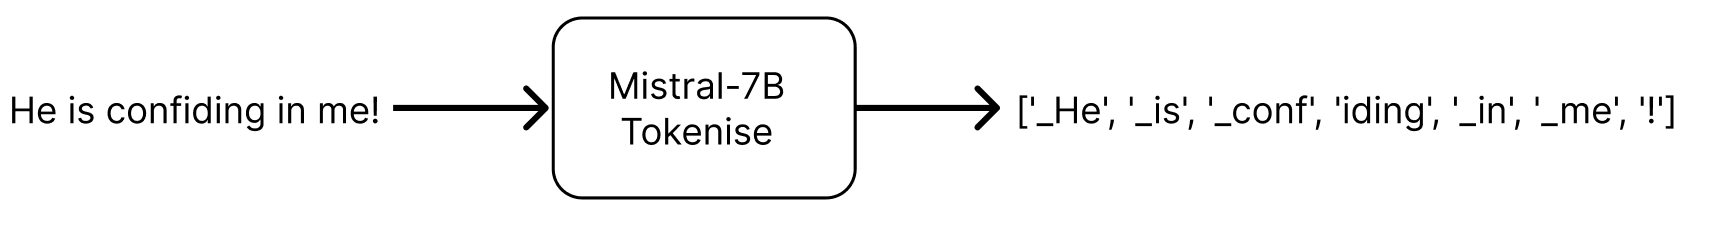
\includegraphics[width=\linewidth]{images/background/tokenisation-process-mistral.png}
                \caption{\emph{(a)}}
                \label{fig:tokenisation-process-mistral}
            \end{subfigure}

            \begin{subfigure}{\textwidth}
                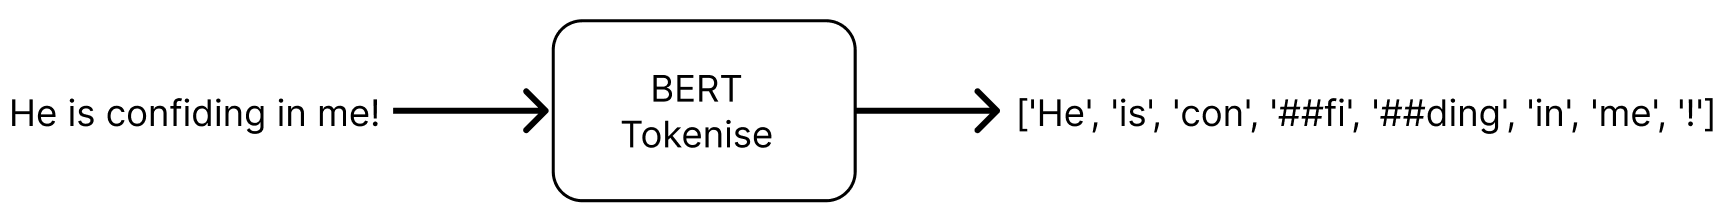
\includegraphics[width=\linewidth]{images/background/tokenisation-process-bert.png}
                \caption{\emph{(b)}}
                \label{fig:tokenisation-process-bert}
            \end{subfigure}

            \caption{Figure visualises the potential differences in tokenisation functions. Figure (a) was completed using the \codefont{Mistral-7B-v0.1} tokeniser \citep{jiang2023mistral}, a BPE tokeniser. Figure (b) was completed using the \codefont{bert-base-uncased} tokeniser \citep{DBLP:journals/corr/abs-1810-04805}, a WordPiece tokeniser.}
            \label{fig:tokenisation-process}
        \end{figure}

        \begin{definition}[Vocabulary]
            A \emph{vocabulary} is the collection of tokens recognised by a tokenisation function.
        \end{definition}

        Importantly for our discussion on watermarking language models, the training of these tokenisation models generates a \emph{unique} vocabulary dependent on the text corpus. The difference in recognised tokens is evident when comparing the lists of tokens in Figure~\ref{fig:tokenisation-process}. The tokenisation uniqueness is propagated through the transformer-based architecture.

        
    
    \subsection{Causal Generation}
        \label{sec:decoder-generation}
        Text generation is treated as a predict-next-token task. The principle idea is to only look at the previous tokens and consider which token is most likely to next appear. This task is known as Causal Generation.

        In an attempt to respect the depth of this paper, I will not be going over the decoder layer. The important thing to note is that the decoder layer will create a matrix of dimensions $C \times E$, where $C$ is the context window and $E$ is the embedding dimension. For the purposes of causal generation, the information about all the previous tokens is within the final row of this matrix.

        % They do not know what word embedding is. Perhaps rephrase this somehow. 
        As can be seen in Figure~\ref{fig:decoding-process}, the final row is taken from the matrix and applied to a linear function. This linear function is another learnable parameter which attempts to undo the word embedding process, bringing the column dimension to match the vocabulary size. 

        \begin{figure}[h]
            \centering
            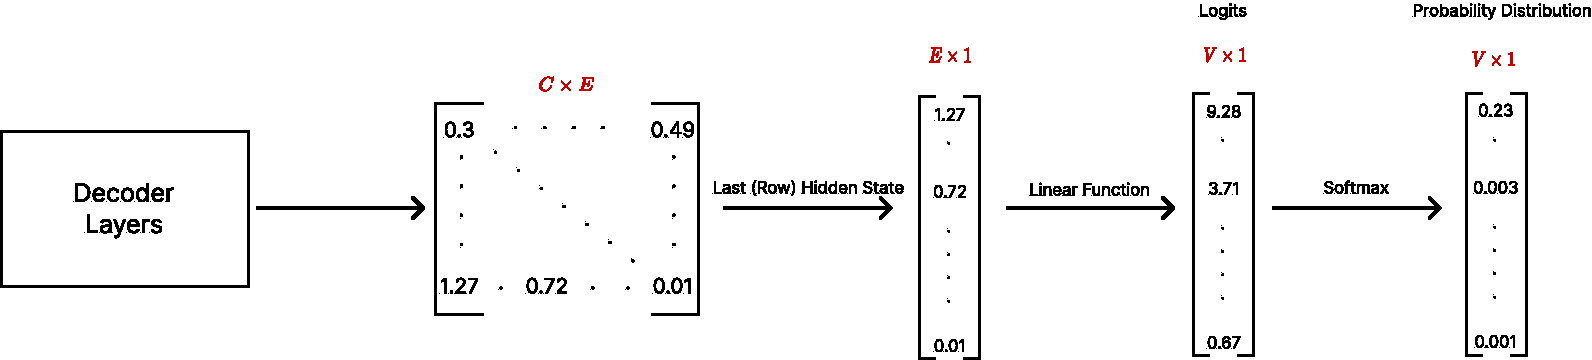
\includegraphics[height=10cm, width=1\linewidth, keepaspectratio]{images/background/decoding-process.pdf}
            \caption{Figure displaying the decoding process ending at the probability distribution, as generative strategies changes how the probability distribution is used. The variables $C$, $E$, $V$ refer to the context window, embedding dimension and vocabulary size respectively. Note that the transformations are not numerically accurate and only showcasing process.}
            \label{fig:decoding-process} 
        \end{figure}

        In the later stages of Figure~\ref{fig:decoding-process}, we apply a linear function to final hidden state. This linear function is a learnable parameter which aims to turn from the embedding dimension to the vocabulary. Importantly, however, is that this linear function is does not perfectly map to a single token. To solve this, we view the output of the function as logits and use these logits to create our probability distribution.
    
        \begin{definition}[Logits]
            Let $p$ be the probability of an event happening. The \emph{logit} is defined as: 
            \begin{equation*}
                \text{logit}(p) = \log\bigg(\frac{p}{1-p}\bigg),
            \end{equation*}
            where logit is defined as $\text{logit}: (0,1) \rightarrow (-\infty, \infty)$.
        \end{definition}
        
        The values of low probability become negative under the logit function. This feature, alongside the wide range of the codomain, provides simple interpretability. As such, logits have become convention within language models.

        The created probability distribution is used for multiple generative strategies which include greedy, beam-generation, multinomial sampling, top-$k$ sampling and nucleus sampling. These differing strategies have different purposes but, importantly, all the methods produce one single token from each probability distribution.

        Logits are important with regards to Section~\ref{sec:maryland-watermark}, where we discuss the method of generating the Maryland Watermark.

    \subsection{Generation Strategies}
        Talk about top-p sampling, multinomial sampling and beam search. 
    
\section{Generating Watermarks}
    \begin{definition}[Watermark]
        A \emph{watermark} is a faint figure or signature designed to represent ownership or authorship.
    \end{definition}

    Watermarks are widely present within society with examples ranging from an American dollar bill to a music producer having an audio tag. 

    \begin{figure}[h]
        \centering
        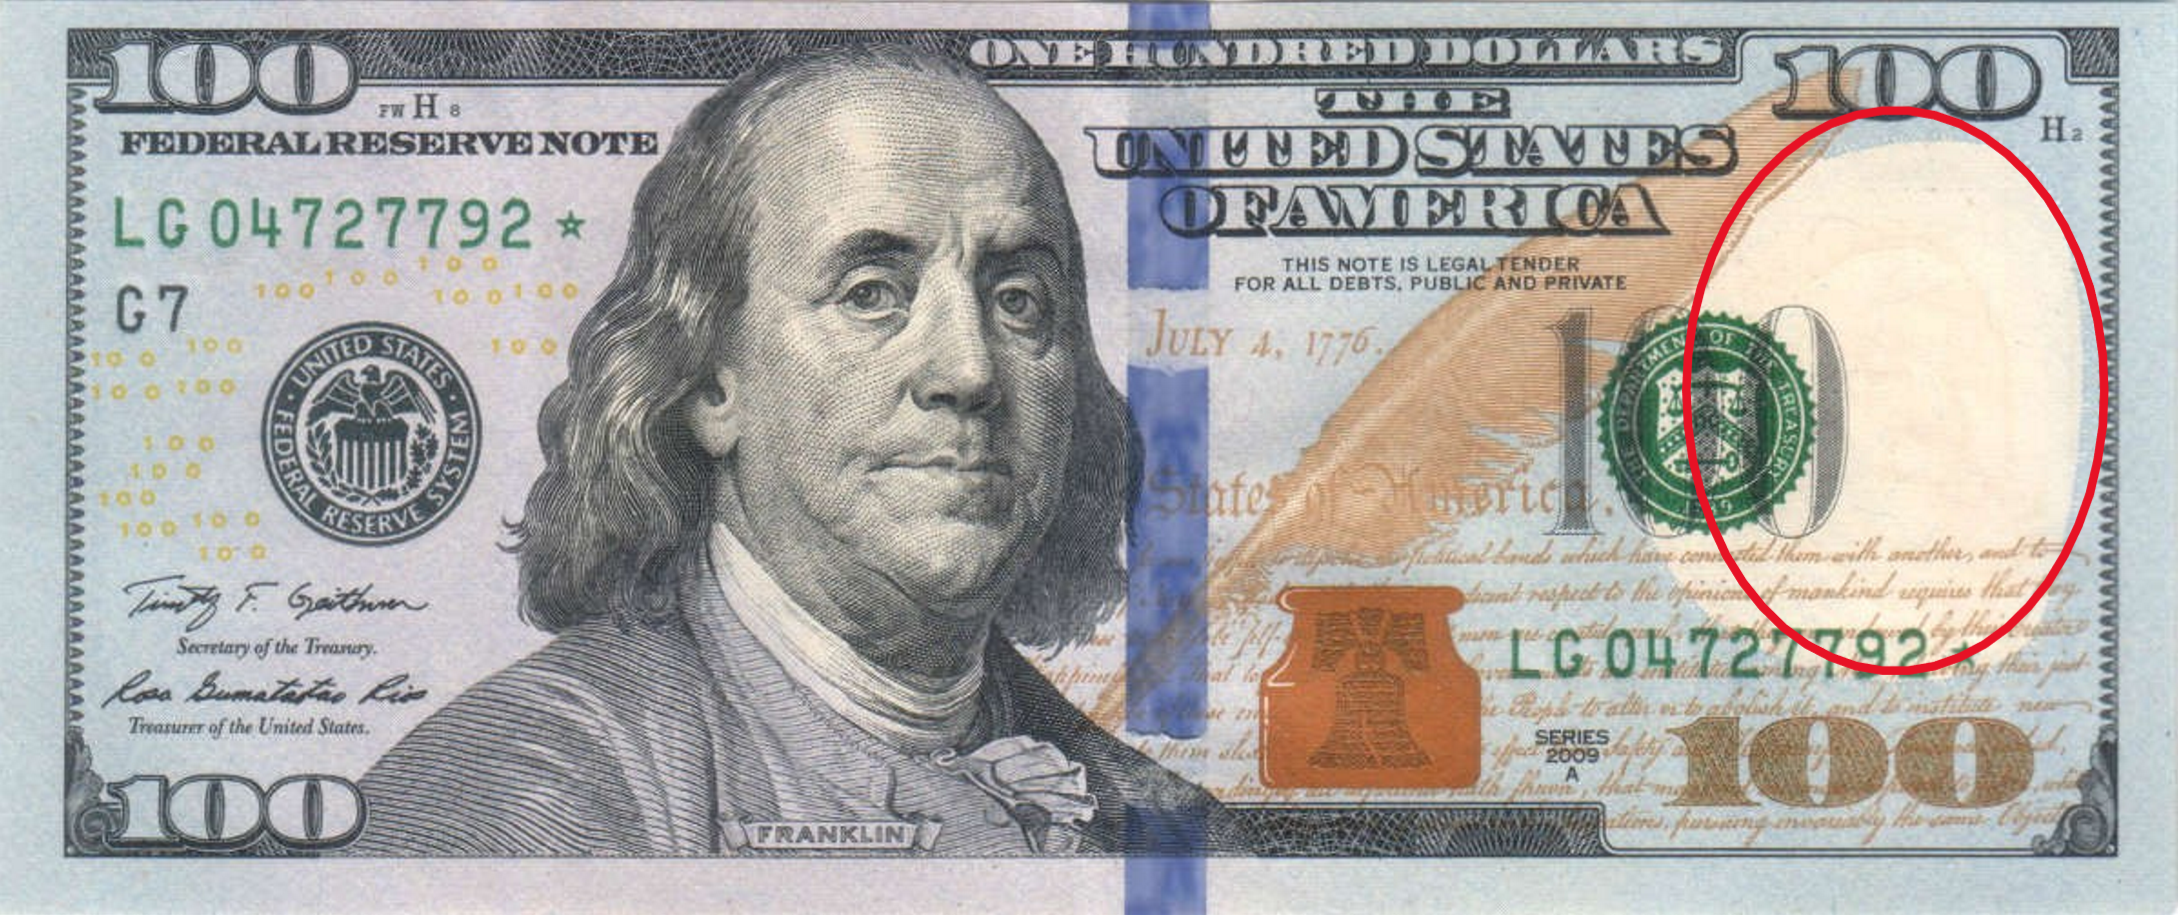
\includegraphics[height=3.5cm, width=1\linewidth, keepaspectratio]{images/background/dbill-highlighted.png}
        \caption{Figure shows an \$100 dollar bill, with a red circle highlighted a watermarked portion. The detection of the highlighted watermark requires holding the bill up to light and revealing a (second) face of Benjamin Franklin.}
         \label{fig:dbill-watermark} 
    \end{figure}

    Watermarks come in many forms, be it a signature: ``Written by Sam Jackson'' or a well-defined pattern of ending every word with the character `n'. In this section, we look towards recent literature which covers more subtle methods of watermarking while attempting to adhere to the primary goals of watermarking.
         
    Given the purpose of watermarking generative content, there are the following primary goals that an AI text watermark aims to achieve:
    \begin{itemize}
        \setlength\itemsep{0.5em}
        \item \textbf{Robust} - Capable of withstanding attempts to remove watermark.
        \item \textbf{Agnostic} - Information beyond generated text is not required for detection.
        \item \textbf{Imperceptible} - The watermark should not be visible, be it a change in quality or a written signature.
    \end{itemize}

    These requirements are specifically designed to encourage universal watermarking techniques due to the constant growing number of large language models and changing architecture decisions.
    
    \subsection{Maryland Watermark}
        \label{sec:maryland-watermark}
        \citet{kirchenbauer2023watermark} proposes a new method of watermarking text which takes advantage of the probabilistic nature of text generation. This section will go over the ideas of the Maryland Watermark, a technique which laid the foundations of watermarks in LLMs at the time of this paper.

        Due to the nature of casual generation, each token is generated procedurally from the vocabulary. The Maryland paper proposes splitting the available vocabulary for each token. The split lists are labelled a \emph{green} list and a \emph{red} list, where green tokens are used for detection. Notably, the splitting is a random sort and partition based on the hash of the last token.

        In particular, there are two primary watermarking techniques, \emph{Hard Watermarking} and \emph{Soft Watermarking}. Hard Watermarking only allows the causal model to select tokens from the green list whereas Soft Watermarking simply increases the probability of the green tokens within the probability distribution. Figure~\ref{fig:soft-watermarking-process} outlines the technique and the change that the Soft Watermarking process makes compared to the generation in Figure~\ref{fig:decoding-process}.

        \begin{figure}
            \centering
            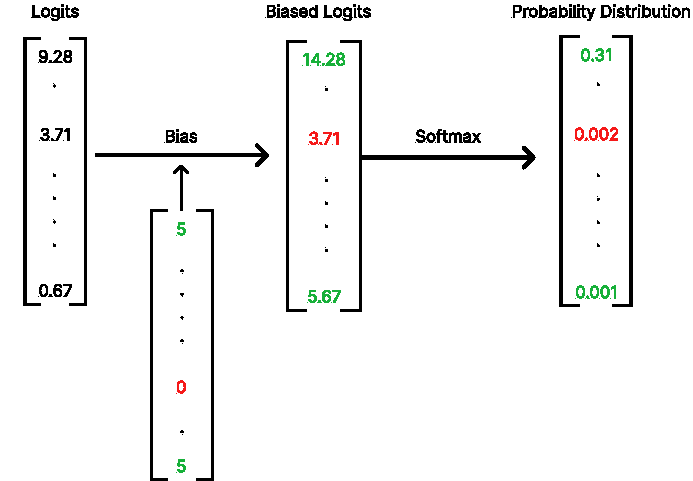
\includegraphics[width=1\linewidth, keepaspectratio]{images/background/biasing-process.pdf}
            \caption{Figure portrays the Soft Watermarking Process highlighting the bias process, where the bias value is 5. Like Figure~\ref{fig:decoding-process}, $C$ is the context window, $E$ is the embedding dimension and $V$ is the vocabulary size. The image ends at the probability distribution, avoiding showing the generation strategy, in order to keep the image abstract. Note that the transformations are not numerically accurate and simply showcasing process, except the biasing.}
            \label{fig:soft-watermarking-process}
        \end{figure}

        As opposed to Hard Watermarking, Soft Watermarking provides parameters that determine the strength of the watermark. The parameters are $\delta$, the logit bias, and $\gamma$ is the fraction of the vocabulary which is the green list. Typical values for $\delta$ and $\gamma$ are within the ranges $[1, 10]$ and $[0.25, 0.5]$, respectively.

        \citet{kirchenbauer2023watermark} provides an analysis on the Soft Watermarking technique, outlining the performance on differing bias and generation strategies. Without describing the necessary metrics, the paper shows that watermarking, with no detection-errors, can be achieved at reasonable strengths of watermarking whilst maintaining quality of the text.
        
    \subsection{Easymark}
        \label{sec:easymark}
        As opposed to complicated and robust watermarking techniques, like described above, \citet{sato2023embarrassingly} beautifully proposes simple watermarks that are not intended to survive bad actors. This portion will briefly go over the watermarks as well as highlight the argument of watermark futility from \citet{sato2023embarrassingly}.

        The provided watermarks are labelled as \emph{Whitemark}, \emph{Variantmark} and \emph{Printmark}. All of the methods are weak to bad actors using attacking techniques such as word-replacement, paraphrasing and homoglyph removal however the method of watermarking leads to no degradation in perplexity. 

        Whitemark suggests changing all the whitespace characters to a particular, non-regular, whitespace character which exists in unicode. This is only a linear-time addition to the generation process and the adjustment is not visible to the human eye.

        Variantmark is focused on Chinese, Japan and Korean (CJK) languages which are not dense with whitespace. As an adjustment for these languages, Variantmark takes advantages of the glyphs within CJK languages containing multiple Unicode sequence points which can be invisibly replaced. The glyph characters contain the same semantic meaning despite a different representation. This process acts as watermarking as the alteration is non-standard.

        Finally, Printmark creates a minute visual change in the letters through similar looking unicode characters. This change is visual enough to appear on printed appear, hence the name, but also subtle enough to not spot unless looking for it. Figure~\ref{fig:fi-ligature} is an example of the technique used for Printmark.

        \begin{figure}[h]
            \centering
            
\includegraphics[width=1\linewidth, height=2.7cm, keepaspectratio]{images/background/inf-ligature.png}
            \caption{Figure showing the similarity between words where the `f' and `i' characters have been changed to the unicode ligature U+FB01, presenting the method used in Printmark.}
            \label{fig:fi-ligature}
            \nocite{infinity-ligatures-pict}
        \end{figure}

        Within the paper, \citet{sato2023embarrassingly} discusses the strength of bad actors and describes a statistical analysis as to why a perfect watermark is impossible. In fact, the paper proposes that it is more prudent to place a low-effort watermark and not place too much confidence within watermarks. 

        Paired with our research questions, our discussion on current watermarking robustness will hopefully bring light to the worthiness of watermarking.
    
    \subsection{Retrieval Defense}
        \citet{krishna2023paraphrasing} proposes a retrieval-based defensive technique, designed to hold strong against paraphrasing attacks. This section will cover the principle ideas and primary results surrounding defense that are discussed in the paper. 

        Contrary to the other watermarking methods, this is a defensive technique that requires no generative-stage changes to the LLMs. The primary idea is to store AI-generated documents into a database and determine if a document is AI-generated by completing a retrieval call into the database.

        % Results at this stage are unknown to reader
        This method achieves significant results with the evaluation taking place over multiple models. Before paraphrasing, retrieval detection has an accuracy of 100\% on 1\% FPR and after strong machine-paraphrasing, there is more than 96\% accuracy across all models. This is compared to the Maryland watermark which achieves 55.8\% accuracy, a starkly lower accuracy.
        
        Notably, for these results, however, is that the retrieval corpus matches exactly the initial generated documents and the retrieval technique is dependent on a reliable database. Furthermore, differing language models may require different databases which could make the retrieval query an expensive cost. 

\section{Attacking Watermarks}
        No matter the robustness of a watermark, methods of successfully attacking are real threats. 

        Within this stage, we will discuss the word-replacement strategy, paraphrasing and translation-attacks. Specifically, we highlight a number of techniques that we will be applying for our method of investigation alongside relevant literature which prove other successful methods of attacking.

    \subsection{Word Replacement}
        A classic and simple technique is \emph{word-replacement}. In this section, I will cover the motivation behind word-replacement as well as an overview of the technique.

        This is perhaps the most primitive form of attacking. As opposed to restructuring a sentence or paragraph, we replace words with suitably appropriate words. We are motivated to complete word-replacement because it is a low-cost approach, comparatively, given the lack of an intensive large language model. Furthermore, the word-replacement algorithm has the potential to remove the so-called `green tokens', reducing the chance of being detected as watermarked.  

        This method is dependent on a Part of Speech (POS) tagger model. A POS model is trained to give grammatical structure to words. This helps us understand how to replace a particular word. Figure~\ref{fig:word-replacement-process} provides a clear outline of the method, containing the Part of Speech tagging. 

        \begin{figure}[h]
            \centering
            
\includegraphics[height=5cm, width=1\linewidth, keepaspectratio]{images/background/word-replacement-process.pdf}
            \caption{Figure displays the word replacement process where 20\% of all words are replaced with similar words, with respect to their part of speech. This process is completed by my word replacement method and the Flair Part of Speech Tagger \citep{akbik2018coling}.}
            \label{fig:word-replacement-process}
        \end{figure}
        
        The major flaw in this method is the lack of semantic understanding. The benefit that transformers provide all large language models is thrown away through the use of this technique and drastically reduces the quality of the text.
        
        Variations of this technique exist, such as only replacing adjectives with respect to the POS tagger. These variations are designed to compensate for the lack of semantic understanding that a word-replacement algorithm has.

        Whilst the method comes with many flaws, this paper will discuss an analysis of this attack, something which is novel amongst current research papers.
    
    \subsection{Paraphrasing}
        Given that the techniques of watermarking are focused around the particular words used within a generated document, we aim to remove those `bad' words, whilst maintaining or improving the clarity of the original meaning. However, without knowing the watermarked words, word-replacement might not be sufficient. 

        In this section, we discuss the solution to our problem with paraphrasing and how that extends into large language models, as well as recent papers surrounding paraphrasing attacks.

        \begin{definition}[Paraphrase]
            \label{def:paraphrase}
            To repeat something written or spoken using different words, often in a humorous form or in a simpler and shorter form that makes the original meaning clearer (Cambridge Dictionary, 2024). % Perhaps I should cite this in references
        \end{definition}

        As can be seen in Example~\ref{example:paraphrase}, we often restructure sentences for clarity which is something that word-replacement is incapable of doing without a degree of semantic understanding.

        \begin{example}
            \label{example:paraphrase}
            The two sentences below are examples of paraphrases.
            \begin{enumerate}[label=(\alph*)]
                \item I take my dog on a walk in Central Park each Wednesday. 
                \item Every Wednesday, I walk my dog in Central Park.
            \end{enumerate}
            These two sentences maintain semantic meaning while holding a different sentence structure. 
        \end{example}

        In recent literature, \citet{krishna2023paraphrasing} discusses the attacks of paraphrasing by providing a paraphrase language model known as DIPPER. Through finetuning, this model is a paragraph-context paraphrase model with variable parameters. These parameters determine the degree of order and lexical change performed by the paraphrasing. 

        Within the DIPPER paper, results are provided in Section 4.1 of the paper which convey the drastically decreasing detection accuracy as the order and lexical parameters increase.
        The paper's highlighted statistic shows that where false detection of human-text as AI-text is at 1\%, the DIPPER paraphraser drops accuracy of DetectGPT from 70.3\% to 4.6\%.

        Similarly, in other literature, \citet{sadasivan2023aigenerated} investigates recursive paraphrasing on watermarked documents with two models, DIPPER and a LLaMa-based chat model. In particular, the analysis takes place on generated documents of approximately 300 tokens. 

        The paper reports results of clear degradation in detection through the iterations of DIPPER-based paraphrasing. With the case where false-detection of human-text as AI-text is at 1\%, the chance that a watermarked document is detected drops from 99.8\% in the original document to 30.9\% in the third paraphrase. This is significant change at minimal cost, as reported by \citet{sadasivan2023aigenerated}, where the cost is discussed with respect to the perplexity metric.

        This paper will be using a variation of the DIPPER model for paraphrasing as well as the recursion concepts as part of our evaluation into the robustness of watermarking. 

    \subsection{Translation-Based Paraphrasing}
        \citet{he2024watermarks} provides a deep investigation into the process of using translation to remove watermarks. As opposed to training a new paraphraser, \citet{he2024watermarks} utilises existing translation models in order to paraphrase. This section will give a brief overview as to how this works and the performance of the technique. 

        As can be seen in Figure~\ref{fig:translation-removal-process}, the principle idea behind translation-based paraphrasing is twice-translation, going to another language and back. 

        \begin{figure}[h]
            \centering
            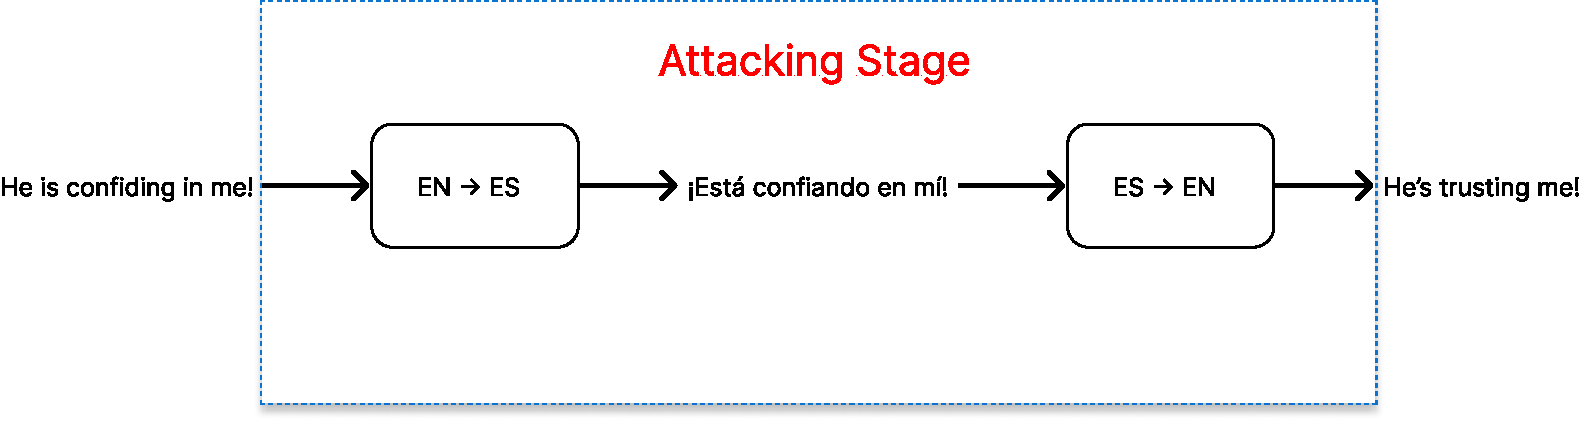
\includegraphics[height=3.5cm, width=1\linewidth, keepaspectratio]{images/background/translation-removal-process.pdf}
            \caption{Figure above displays the translation attacking process with twice translation involving English and Spanish. Translations were completed with the \texttt{opus-mt-en-es} and \texttt{opus-mt-es-en} models respectively \citep{TiedemannThottingal:EAMT2020}.}
            \label{fig:translation-removal-process}
        \end{figure}
        
        This method is particularly effective because the architecture behind paraphrasing and translation is the same: Sequence-to-Sequence (Seq2Seq). The Seq2Seq architecture is a decoder which has access to all the tokens in a document, not just the previous ones. This drastically improves the performance of LLMs on tasks like summarisation as it takes different context into account. 

        \citet{he2024watermarks} outlines clear results which portray the efficacy of this technique. A highlighted result is, in the case of false-detection of human-text as AI-text is at 10\%, the chance that a watermarked document is detected drops from 99.2\% to 21.3\%. This is a significant change and shows that the translation attacks bring the performance of a random classifier. 

        An important note is that this result is retrieved from analysis of the watermark at a weaker strength than this paper's watermark. This means that the detection accuracy would be greater if the watermark was of similar strength to ours. Furthermore, since the false detection is at 10\% which is greater than previously mentioned results, the detection accuracy is greater whilst at a greater risk.

    \subsection{Other Techniques}
        Despite the number of these techniques, there does exist others that I will not be able to provide a deep background into within this paper.

        A technique which was previously mentioned was \emph{homoglyph removal}. This technique is used to counter embedding watermarks through ASCII and Unicode characters, a perfect counter to the watermarking concepts in Section~\ref{sec:easymark}. The technique consists of a script which tests each character against Unicode pairs, replacing uncommon variations of a character to the norm. 

        In the spirit of counters, a counter to the Maryland technique is \emph{prompt engineering}. This technique is nuanced to the application of the Maryland watermark however I will attempt to cover it in a brief sentence. The Maryland Watermark generates the split list based on the previous token so the order and choice of word is particularly important. Through manipulating the prompt, the output can be instructed to replace all the whitespace characters with an emoji and lead to fixing the splitting of the lists. Consequently, the emojis can be removed and the detection can no longer deduce the green and red lists. Without the lists, the watermark cannot be found. 

        Both of these techniques are particularly effective counters but they will not be further discussed in this paper as they are only applicable to certain watermarks. 

\section{Approach}  
    Following all of this background, we summarise the primary points that will be used for the rest of our paper. Within the rest of this paper, we shall be generating documents and attacking them through three primary methods.

    Our attacking methods consist of:
    \begin{itemize}
        \setlength\itemsep{0.5em}
        \item \textbf{Paragraph-Based Paraphrasing}: Paraphrasing the entire document, supplying the entire context. 
        \item \textbf{Sentence-Based Paraphrasing}: Paraphrasing each sentence within a document, only supplying context of the given sentence.
        \item \textbf{Word Replacement}: Changing words within the document to similar words.
    \end{itemize}

    % Discuss the defensive phase as well as evaluation? 
    
    \subsection{Problem Phrased}
        Our problem can be succinctly defined in the following question: ``To what extent are modern-day watermarking techniques robust against bad actors?''

        This paper breaks down that question into 3 smaller sub-questions. These sub-questions form our research questions for the paper and what we aim to understand.
        \begin{enumerate}[label={\textbf{RQ\arabic*}:}, leftmargin=4em]
            \label{sec:research-questions}
            \item Does recursive paraphrasing provide more effective removal of a watermark?
            \item Is sentence-based paraphrasing sufficient compared to recursive paraphrasing?
            \item Is a simple word replacement algorithm sufficient to remove the watermark?
        \end{enumerate}

%====================================================================================================
    
\chapter{Methods}
\textbf{What did you do to implement this idea, and what technical achievements did you make?}

With the aim of understanding the robustness of watermarks in generative text, we discuss our method that takes us from the generation of watermarked documents to the evaluation of attacked documents.

\section{Overarching Approach}
    Before detailing all the design choices, I present the overarching implementation of our research method to aid in following along amongst the choices. The visual in Figure~\ref{fig:method-flow-chart} is provided to further assist in understanding the approach.

    \begin{figure}[h]
        \centering
         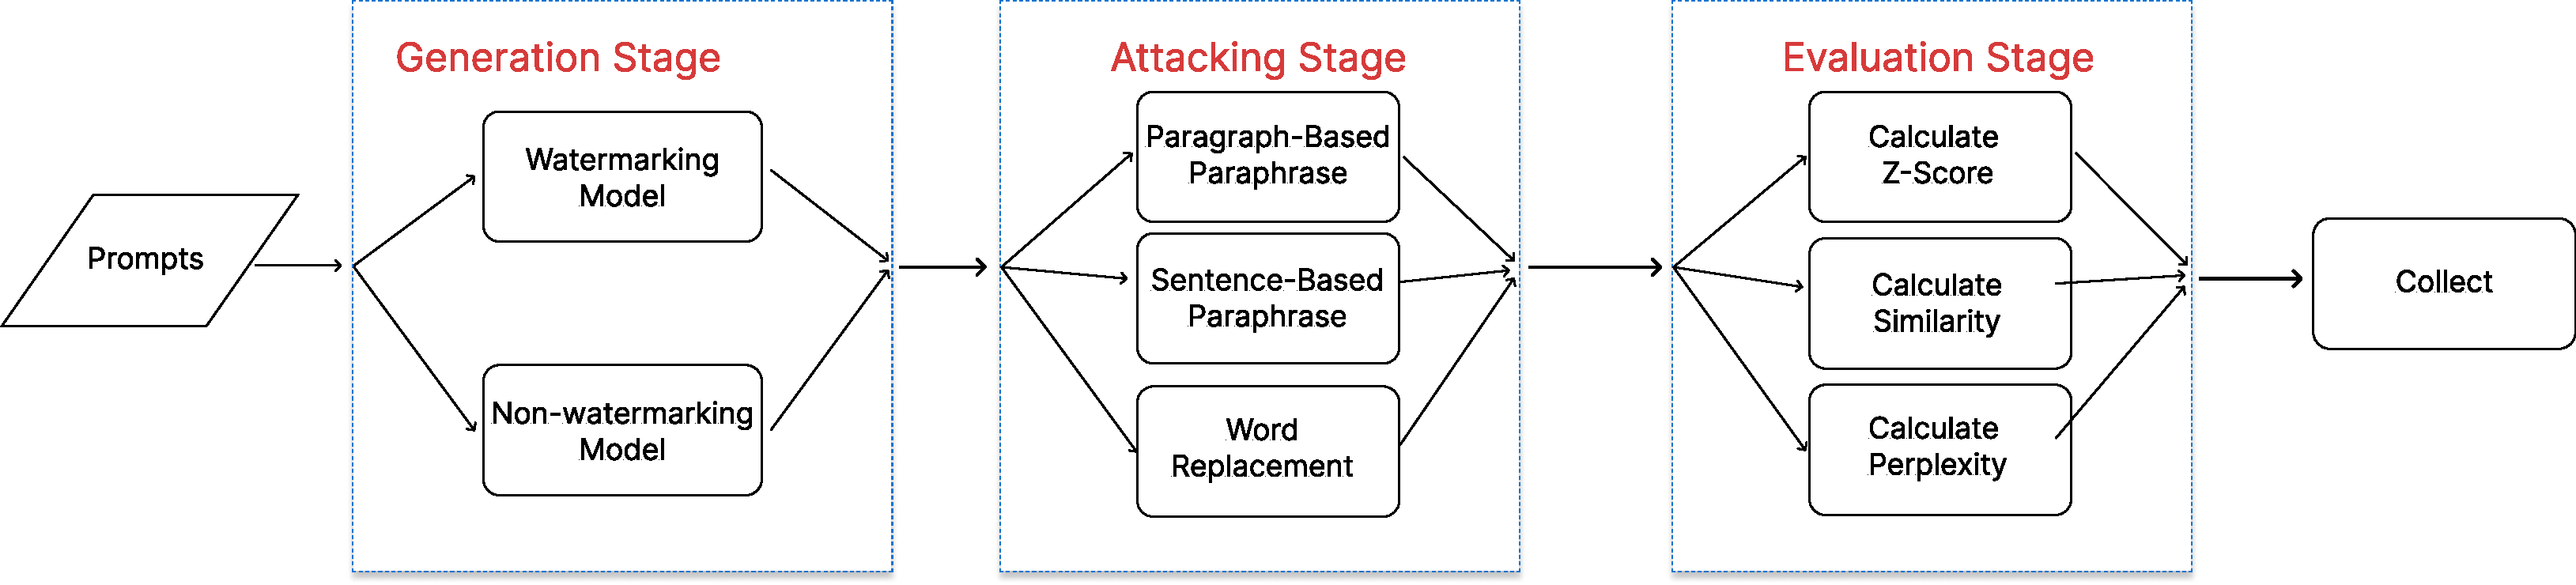
\includegraphics[height=10cm, width=1\linewidth, keepaspectratio]{images/methods/research-process.pdf}
        \caption{Figure displaying the research processing, highlighted into the stages.}
        \label{fig:method-flow-chart} 
    \end{figure}
    
    The approach begins with creating watermarked documents through a large language model, given a dataset of prompts. These watermarked documents will be paired alongside real essays, written by humans, to help ensure the quality of the watermark.

    Consequently, these essays are passed through our chosen attacking methods. These attacking methods will be two variants of paraphrasing as well as word-replacement. 

    Finally, we will evaluate the watermark quality of all the documents, which will include all the attacked documents as well as the original documents. There will be two primary evaluation stages with further evaluation metrics to help display the results in a meaningful representation.

\section{Generation Stage}
    \subsection{Dataset}    
        To generate our watermarked documents, prompts had to be provided to a causal language model. To match our causal model, the prompts were selected to be instructions. The chosen dataset ended up being a collection of essay prompts, paired with real student essays. 
    
        Kaggle, a data science platform, hosted a competition focused on detecting AI generated text \citep{llm-detect-ai-generated-text}. The competition led to the creation of model-finetuning augmenting datasets. One such augmenting dataset is known as the DAIGT dataset, produced by \citet{Paullier2023-rx}, and is the dataset that will be used.

        The associated student essays were scraped from a separate Kaggle competition \citep{feedback-prize-english-language-learning}, guaranteeing the humanity of the essays.

        The dataset is composed of four columns: \emph{id}, \emph{text}, \emph{instructions}, \emph{source\_text}. There is 2421 documents within the dataset. The \emph{source\_text} column is misleading as this column is generated by ChatGPT, as per \citet{Paullier2023-rx}, contrary to what the name suggests. 

        \begin{table}[h]
            \centering
            \small 
            \begin{tabular}{@{}l|p{0.25\linewidth}|p{0.25\linewidth}|p{0.25\linewidth}@{}}
                \toprule
                id & text & instructions & source\_text \\ \midrule
                6060D28C05B6 & Some schools in United States ofter classes from home because is good option to students . Some scho... & Task: Write a persuasive essay on whether or not classes from home should be offered as an option f... & When considering the pros and cons of attending classes from home, there is no doubt that there are... \\ \cmidrule(r){1-4}
                60623DB5DE7A & Four-day work week, a remarkable idea to conserve energy and resources, some businesses have adopted... & Task: Research the advantages and disadvantages of a four-day school week and write an essay to det... & One of the primary arguments for implementing a four-day school week is the potential cost savings.... \\ \bottomrule
            \end{tabular}
            \captionsetup{width=.95\textwidth}
            \caption{The above table displays 2 of the existing 2421 rows within the DAIGT dataset, where columns are cut for brevity and readability.}
            \label{table:dataset-sample} 
        \end{table}

        Within other literature, the method of generating watermarked documents was auto-generative prompting. This style of prompting influences model and dataset choice.
    
        Initial experiments with auto-generative prompting were headed with the dataset created by \citet{Signal1M2016}, a dataset of 1 million news articles. 
        Given the popularity and use of instruct models, I chose to focus on the instruct-style datasets as opposed the typical auto-generative style. This focus away from auto-generative prompting is not investigated amongst current literature which could lead to differences in watermarking quality.
        
    \subsection{Model}
        In order to generate the watermark, we look for an appropriate model. Current literature is typically using auto-generative and chat models \citep{pang2024attacking, liu2024adaptive, kirchenbauer2023watermark, sadasivan2023aigenerated} so this paper will look towards other models.

        Specifically, this paper will focus on an Instruct model, a model which is finetuned towards dealing with instruct-style prompts. The chosen model is a Mistral model,\codefont{Mistral-7B-Instruct-v0.2} \citep{jiang2023mistral}, which is a 7 billion parameter model.

        From Figure~\ref{fig:prompting-method}, the prompting method is catered towards an Instruct response, with an actual essay prompt from our chosen dataset.
        
        \begin{figure}[h]
            \centering
            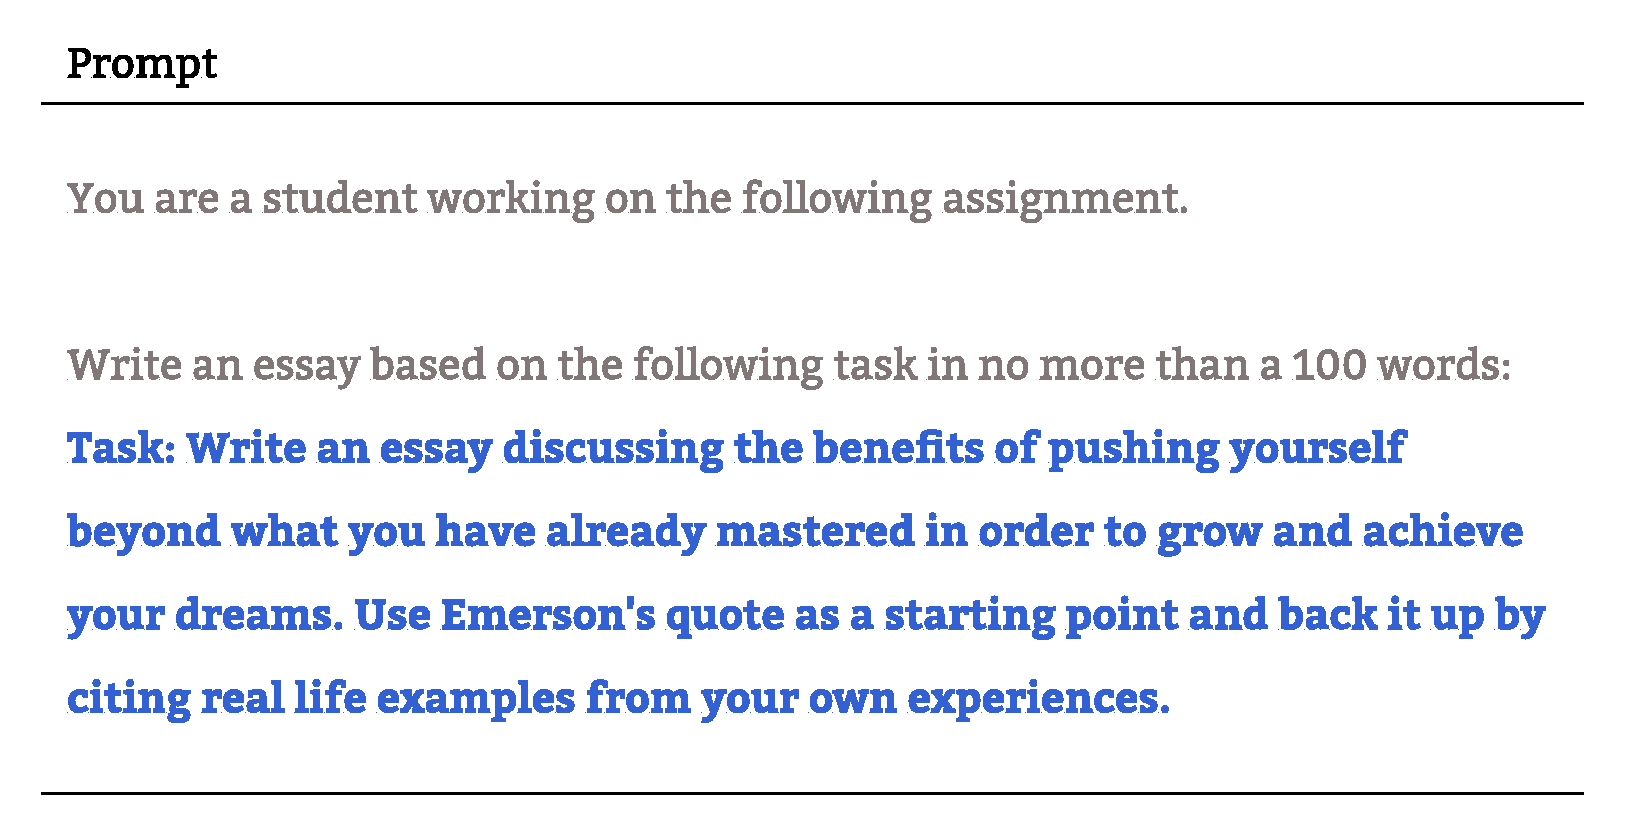
\includegraphics[height=4cm, width=1\linewidth, keepaspectratio]{images/methods/prompt-template.pdf}
            \caption{Figure portraying the prompting method used for the generation of watermarked essays, where \textbf{\{chosen\_task\}} denotes a document from the DAIGT dataset.}
            \label{fig:prompting-method}
        \end{figure}

        The chosen generation strategy was multinomial sampling, with the max number of new tokens generated set at 7500, to allow for potentially large documents.
        
    \subsection{Watermark}    
        \label{sec:watermark-implementation}
        Our chosen application of watermarking will be the Maryland Watermark, outlined in Section~\ref{sec:maryland-watermark}. Specifically, we will be using the Soft Watermarking method which better permits more realistic language generation. 

        The Maryland Watermark was the ideal watermark as it is the original paper on the logit-manipulation-based watermarking. Other watermarking techniques are present, such as Easymark from Section~\ref{sec:easymark} or a Semantics-based watermark \citep{hou2024ksemstamp}, however these watermarks are not implemented to respect the breadth of this paper. 

        Our implementation is completed using the HuggingFace Python library \citep{wolf-etal-2020-transformers}, alongside code provided by \citet{kirchenbauer2023watermark}. This library provides an interface to the language model as well as the ability to manipulate logits at the generation stage, prior to the creation of the probability distribution, as outlined in Figure~\ref{fig:soft-watermarking-process}. 

        Specifically, we choose our bias and green list fraction to be $\delta = 5$ and $\gamma = 0.25$ respectively. This means that for the generation of each token, a quarter of the vocabulary are `green' tokens. Similarly, those `green' tokens will have a bias of 5 added to them. These parameters are in line with results from \citet{kirchenbauer2023watermark} and reflect a strong watermark that maintains a reasonable degree imperceptibility.

\section{Attacking Stage}
    In this section, I will be going over our attacking technique. In order to understand the robustness of watermarks, it is necessary to attempt watermark removal with a diverse range of methods. 

    As highlighted in Figure~\ref{fig:method-flow-chart}, we choose to paraphrase attack with a sentence-based and paraphrase-based paraphraser. Furthermore, we apply our word-replacement algorithm as an attacking method. All of the prior methods will be discussed in this section, in the listed order.

    The mentioned techniques precisely cover our research questions, \textbf{RQ1}, \textbf{RQ2} and \textbf{RQ3}, which helps us answer our overarching questions of watermark robustness.

    \subsection{Paragraph-Based Paraphrasing}
        Our attacking approach of paraphrasing with respect to the paragraph is based on the idea of supplying the maximal amount of context. With more context, the model is afforded greater potential to gleam the semantic meaning of a document. 
    
        To create a paragraph-based paraphraser, we choose a model with the same architecture as a translation model. \citet{krishna2023paraphrasing} proposes precisely this model, known as DIPPER. In fact, the paper discusses finetuning from dataset generation to a finetuned model. Unfortunately, due to computational constraints, we could not use the given model. As a result, we choose to create our own model, with the principles from this initial paper. For brevity, I will refer to this model as \emph{$p$-paraphraser}.
        
        Specifically, we finetune a Sequence-to-Sequence (Seq2Seq) model with a dataset of paragraph pairs. We decide upon one of Google's T5 models, models designed for being refined on specific tasks. We chose to use \codefont{t5-efficient-large-nl32}. The suffix of this model refers to the number of transformer blocks, where 32 is larger than the norm. The large number of transformer block adheres to a Deep-Narrow architecture, a recommendation from \citet{tay2022scale}, the paper which recommended these models.

        To construct our dataset, we lend from \citet{krishna2023paraphrasing} and use their dataset, which I will refer to as kPar3. Par3 \citep{Par3_2022} is the predecessor to kPar3, prior to processing, and presents paragraph-aligned translations of books. Figure~\ref{fig:par3-collection-process} provides a visual description of how the data is collected.

        \begin{figure}[h]
            \centering
            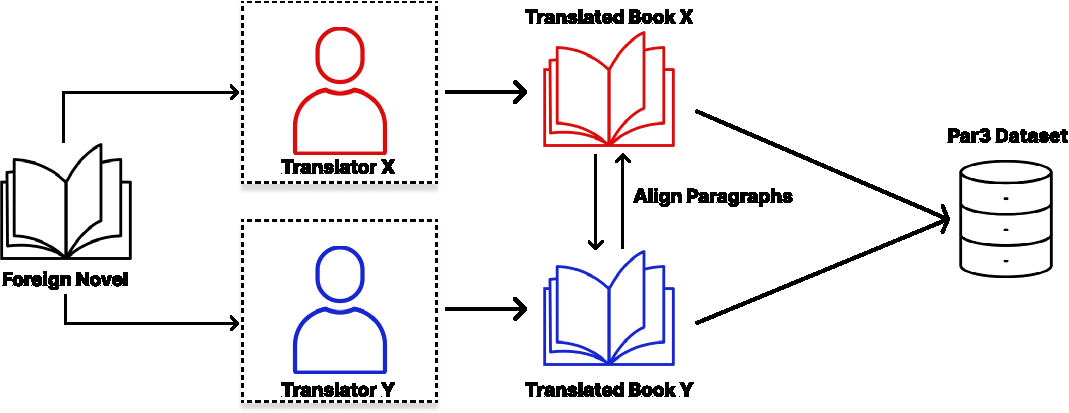
\includegraphics[width=1\linewidth, height=5cm, keepaspectratio]{images/methods/par3-collection-explanation.pdf}
            \caption{Figure describing how the Par3 data is created and produced. Figure is outlining that a famous book is translated by multiple distinct people. The respective translation paragraphs are aligned with eac
         other and considered paraphrases.}
            \label{fig:par3-collection-process}
        \end{figure}

        The kPar3 dataset created documents that contained $\sim$6,000,000 paraphrase pairs, split between Google translated and the human translated described above. Within each section, there is further nondescript subsections. These subsections are composed of documents which provide context to the paraphrase and those that which do not. The structure of the dataset is described in Figure~\ref{fig:kpar3-structure}. Each document starts with the arguments \emph{lexical} (L) and \emph{order} (O), as seen in Figure~\ref{fig:kpar3-sample-comparison}, where each argument only has values from the set \{0, 20, 40, 60, 80, 100\}. These arguments are included to impose an understanding of paraphrasing strength in the model.

        \begin{figure}[h]
            \centering
            \includegraphics{images/methods/kpar3-structure.pdf}
            \caption{Figure describing how the kPar3 is structured}
            \label{fig:kpar3-structure}
        \end{figure}
        
        To respect the time it will take to train $p$-paraphraser, we sample the kPar3 dataset. Importantly, we only sample from paraphrase pairs with no context. A visual comparison between context and non-context paraphrase is provided in Figure~\ref{fig:kpar3-sample-comparison}. Non-context pairs were chosen to avoid finding an appropriate context-split within a document to be paraphrased. Furthermore, by creating a context-split, the available text to be paraphrased is reduced. However, it is worth noting that context-paraphrases perform better in the original paper \citep{krishna2023paraphrasing}.
            
        \begin{figure}[h]
            \centering
            \captionsetup[subfigure]{labelformat=empty}
            \begin{subfigure}{.5\textwidth}
                \centering
                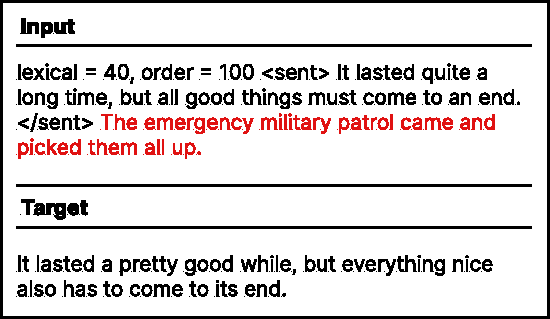
\includegraphics[width=.9\linewidth]{images/methods/kpar3-context-sample.pdf}
                \caption{\emph{(a)} Context Sample}
                \label{fig:kpar3-context}
            \end{subfigure}%
            \begin{subfigure}{.5\textwidth}
                \centering
                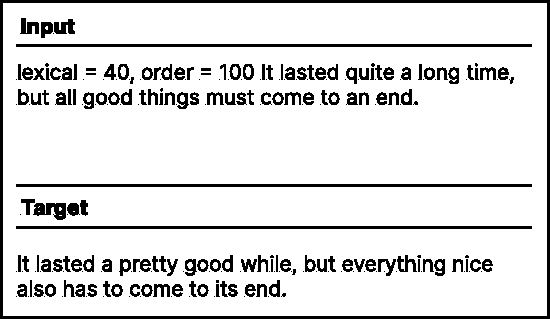
\includegraphics[width=0.9\linewidth]{images/methods/kpar3-non-context-sample.pdf}
                \caption{\emph{(b)} Non-context Sample}
                \label{fig:kpar3-non-context}
            \end{subfigure}
            \caption{Figure displays comparison between a paraphrase pair with context (a), and a paraphrase without context (b). The context portion in (a) is highlighted red for clarity. Furthermore, in (a), the <sent> tags denotes the text to be paraphrased. The target section refers to the desired output of text. Our dataset sample only contains examples like shown in (b). The terms `lexical' and `order' refer to the parameters used for determining paraphrase strength.}
            \label{fig:kpar3-sample-comparison}
        \end{figure}
        
        The original paper trains the model on the entire kPar3 dataset, taking between 384-768 GPU hours. Incapable of replicating the same compute periods, the finetuned model that I present is trained on our sampling of 100,000 documents, taking 14 GPU hours. Further specifications into the training arguments are provided as an appendix. 

        Finally, to attack our documents, we apply paraphrasing attacks on the entire document with the parameters L40 and O20, describing a moderate paraphrase. Similarly, our generation strategy is top-$p$ sampling, as suggested in the original paper \citep{krishna2023paraphrasing}. The paraphrasing is repeatedly recursively to assist in our understanding of \hyperref[sec:research-questions]{\textbf{RQ1}}.

        
    \subsection{Sentence-Based Paraphrasing}
        Opposing the prior method, we aim to separate the paragraph into sentences here and paraphrase each sentence independently. In this section, I will cover the algorithm and model that helps us answer \hyperref[sec:research-questions]{\textbf{RQ2}}.

        With regards to the model, we chose a model known as the \codefont{ChatGPT Paraphraser}\citep{chatgpt_paraphraser}. Similar to the paragraph model previously described, this is a model built off of T5, \codefont{T5-base} specifically. The paraphraser is trained on a synthetic dataset of paraphrases produced by ChatGPT, hence the name. As before, for brevity, I will refer to this model as \emph{$s$-paraphraser}.

        This model was chosen due to a lack of sentence-based models within research literature and consequent popularity of the model within the HuggingFace platform.

        As our attacking method, we complete sentence-based tokenisation with the help of the Natural Language Toolkit (NLTK) \citep{bird2009natural}. Each sentence is separated and passed to our paraphaser, similarly using top-$p$ sampling. The paraphrased sentences are connected together once more, as sentences, maintaining their order.

        The existence of $s$-paraphraser is precisely what we need, alongside our paragraph-based paraphaser, in order to answer \hyperref[sec:research-questions]{\textbf{RQ2}}.
    
    \subsection{Word Replacement}
        In order to answer \hyperref[sec:research-questions]{\textbf{RQ3}}, we attempt attacking with the use of a word-replacement algorithm. Within this section, I will be discussing the implementation of the algorithm as well as the particular variations that we choose to evaluate.

        The algorithm is dependent on appropriately identifying the grammatical nature of each word, as to find an apt replacement. An immediate solution to this is available in the form of Flair's POS Tagger \citep{akbik2018coling}, which is a low-cost model that provides grammatical insight into a sentence.

        The POS tagger is paired with WordNet \citep{wordnet1998fellbaum} which recognises 155,327 distinct words. Linked to these recognised words, there is 117,597 sets of synonyms, known as Synsets. Notably, two words can be linked to the same Synset. The actual statistics of available words is added as an appendix.

        With the knowledge of a word and its grammatical structure, we can apply word-replacement by searching the related Synset and selecting an option from here. Our selection from the Synset is a random sample, as the set is unordered. This synonym choice could be improved by picking the most similar word, according to word embedding model, such as Word2Vec.

        Hence, we can summarise our algorithm as follows:
        \begin{enumerate}
            \item \textbf{Tagging}: Grammatically tag the document with Flair's POS.
            \item \textbf{Select Words}: Select words to replace based on percentage or word-type.
            \item \textbf{Find Synonyms}: With respect to the selected words and grammar, collect potential synonyms.
            \item \textbf{Choose Synonym}: Randomly sample a choice from the synonym set.
            \item \textbf{Rebuild Document}: Rebuild the document, replacing the chosen words.
        \end{enumerate}

        The selection outlined as Step (2) is where we introduce algorithm variations. With a tagged document, we could randomly replace a given percentage of the document. This has flaws as WordNet is not accustomed to dealing with verb replacement of differing tenses. To deal with this, we could choose to replace all the nouns or adjectives. However, importantly, by limiting to certain grammar, we risk not replacing many words.

        In this paper, we choose to attack with a \emph{noun-replacement} approach as well as \emph{25\% of words replacement} approach. Noun-replacement was chosen as the library recognises more nouns than any other type of word combined, as mentioned in WordNet stats found in the appendix. The percentage attack is selected to match the green list fraction, as mentioned in Section~\ref{sec:watermark-implementation}. 

        The attack of this algorithm will provide exactly the results necessary to discuss \hyperref[sec:research-questions]{\textbf{RQ3}} effectively.

\section{Evaluation Stage}
    The most important part of our method stage is our evaluation. This section will discuss our evaluation strategy as well as the necessary metrics for understanding our results. The approach we have taken to evaluation is graphically outlined in Figure~\ref{fig:method-flow-chart}. 
    
    Our main topics are detection, similarity and perplexity. These topics are intended measure watermark strength, paraphrase quality and text quality respectively. 
    
    \subsection{Watermark Detection}
        \begin{itemize}
            \item Z-score definition
            \item Type-I, Type-II errors / TPR, FNR definitions
            \item AUROC 
            \item Maryland detection implementation 
        \end{itemize}
        
    \subsection{Document Similarity}
        \begin{itemize}
            \item Paraphrase similarity vs paragraph similarity.
            \item Example to showcase issues.
            \item Our implementation of paraphrase similarity.
        \end{itemize}

    \subsection{Perplexity Measure}
        \begin{itemize}
            \item Perplexity definition
            \item Model used for perplexity and why
        \end{itemize}

\section{Collection Stage}
    \subsection{Results}
        Discussion here about expected results size. Dataframe size and whatnot.


% \section{General points}
% These points apply to the whole dissertation, not just this chapter.

% FIGURES --------------------------------------------------------
% \subsection{Figures}
% \emph{Always} refer to figures included, like Figure \ref{fig:relu}, in the body of the text. Include full, explanatory captions and make sure the figures look good on the page.
% You may include multiple figures in one float, as in Figure \ref{fig:synthetic}, using \texttt{subcaption}, which is enabled in the template.



% Figures are important. Use them well.
% \begin{figure}
%     \centering
%     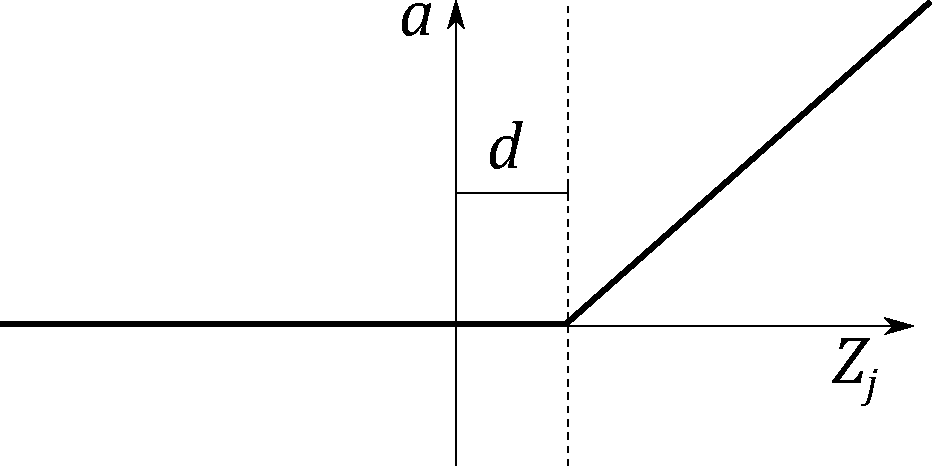
\includegraphics[width=0.5\linewidth]{images/relu.pdf}    

%     \caption{In figure captions, explain what the reader is looking at: ``A schematic of the rectifying linear unit, where $a$ is the output amplitude,
%     $d$ is a configurable dead-zone, and $Z_j$ is the input signal'', as well as why the reader is looking at this: 
%     ``It is notable that there is no activation \emph{at all} below 0, which explains our initial results.'' 
%     \textbf{Use vector image formats (.pdf) where possible}. Size figures appropriately, and do not make them over-large or too small to read.
%     }

%     % use the notation fig:name to cross reference a figure
%     \label{fig:relu} 
% \end{figure}

% \begin{figure}
%     \centering
%     \begin{subfigure}[b]{0.45\textwidth}
%         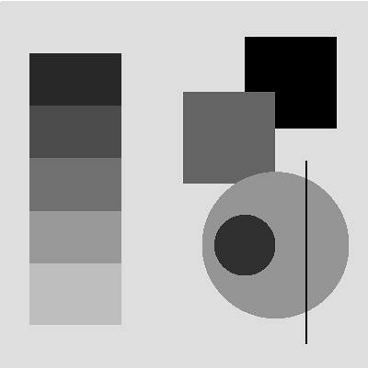
\includegraphics[width=\textwidth]{images/synthetic.png}
%         \caption{Synthetic image, black on white.}
%         \label{fig:syn1}
%     \end{subfigure}
%     ~ %add desired spacing between images, e. g. ~, \quad, \qquad, \hfill etc. 
%       %(or a blank line to force the subfigure onto a new line)
%     \begin{subfigure}[b]{0.45\textwidth}
%         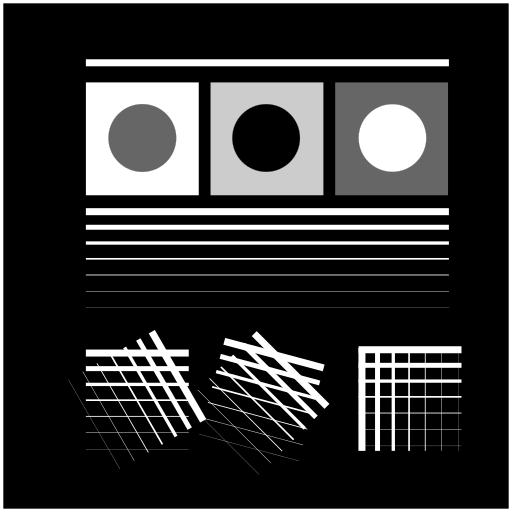
\includegraphics[width=\textwidth]{images/synthetic_2.png}
%         \caption{Synthetic image, white on black.}
%         \label{fig:syn2}
%     \end{subfigure}
%     ~ %add desired spacing between images, e. g. ~, \quad, \qquad, \hfill etc. 
%     %(or a blank line to force the subfigure onto a new line)    
%     \caption{Synthetic test images for edge detection algorithms. \subref{fig:syn1} shows various gray levels that require an adaptive algorithm. \subref{fig:syn2}
%     shows more challenging edge detection tests that have crossing lines. Fusing these into full segments typically requires algorithms like the Hough transform.
%     This is an example of using subfigures, with \texttt{subref}s in the caption.
%     }\label{fig:synthetic}
% \end{figure}

% \clearpage

% EQUATIONS --------------------------------------------------------
% \subsection{Equations}

% Equations should be typeset correctly and precisely. Make sure you get parenthesis sizing correct, and punctuate equations correctly 
% (the comma is important and goes \emph{inside} the equation block). Explain any symbols used clearly if not defined earlier. 

% For example, we might define:
% \begin{equation}
%     \hat{f}(\xi) = \frac{1}{2}\left[ \int_{-\infty}^{\infty} f(x) e^{2\pi i x \xi} \right],
% \end{equation}    
% where $\hat{f}(\xi)$ is the Fourier transform of the time domain signal $f(x)$.

% ALGORITHMS --------------------------------------------------------
% \subsection{Algorithms}
% Algorithms can be set using \texttt{algorithm2e}, as in Algorithm \ref{alg:metropolis}.

% % NOTE: line ends are denoted by \; in algorithm2e
% \begin{algorithm}
%     \DontPrintSemicolon
%     \KwData{$f_X(x)$, a probability density function returing the density at $x$.\; $\sigma$ a standard deviation specifying the spread of the proposal distribution.\;
%     $x_0$, an initial starting condition.}
%     \KwResult{$s=[x_1, x_2, \dots, x_n]$, $n$ samples approximately drawn from a distribution with PDF $f_X(x)$.}
%     \Begin{
%         $s \longleftarrow []$\;
%         $p \longleftarrow f_X(x)$\;
%         $i \longleftarrow 0$\;
%         \While{$i < n$}
%         {
%             $x^\prime \longleftarrow \mathcal{N}(x, \sigma^2)$\;
%             $p^\prime \longleftarrow f_X(x^\prime)$\;
%             $a \longleftarrow \frac{p^\prime}{p}$\;
%             $r \longleftarrow U(0,1)$\;
%             \If{$r<a$}
%             {
%                 $x \longleftarrow x^\prime$\;
%                 $p \longleftarrow f_X(x)$\;
%                 $i \longleftarrow i+1$\;
%                 append $x$ to $s$\;
%             }
%         }
%     }
    
% \caption{The Metropolis-Hastings MCMC algorithm for drawing samples from arbitrary probability distributions, 
% specialised for normal proposal distributions $q(x^\prime|x) = \mathcal{N}(x, \sigma^2)$. The symmetry of the normal distribution means the acceptance rule takes the simplified form.}\label{alg:metropolis}
% \end{algorithm}

% PSEUDOCODE RULES --------------------------------------------------------
% \begin{table}[]
%     \caption{The standard table of operators in Python, along with their functional equivalents from the \texttt{operator} package. Note that table
%     captions go above the table, not below. Do not add additional rules/lines to tables. }\label{tab:operators}
%     %\tt 
%     \rowcolors{2}{}{gray!3}
%     \begin{tabular}{@{}lll@{}}
%     %\toprule
%     \textbf{Operation}    & \textbf{Syntax}                & \textbf{Function}                            \\ %\midrule % optional rule for header
%     Addition              & \texttt{a + b}                          & \texttt{add(a, b)}                                    \\
%     Concatenation         & \texttt{seq1 + seq2}                    & \texttt{concat(seq1, seq2)}                           \\
%     Containment Test      & \texttt{obj in seq}                     & \texttt{contains(seq, obj)}                           \\
%     Division              & \texttt{a / b}                          & \texttt{div(a, b) }  \\
%     Division              & \texttt{a / b}                          & \texttt{truediv(a, b) } \\
%     Division              & \texttt{a // b}                         & \texttt{floordiv(a, b)}                               \\
%     Bitwise And           & \texttt{a \& b}                         & \texttt{and\_(a, b)}                                  \\
%     Bitwise Exclusive Or  & \texttt{a \textasciicircum b}           & \texttt{xor(a, b)}                                    \\
%     Bitwise Inversion     & \texttt{$\sim$a}                        & \texttt{invert(a)}                                    \\
%     Bitwise Or            & \texttt{a | b}                          & \texttt{or\_(a, b)}                                   \\
%     Exponentiation        & \texttt{a ** b}                         & \texttt{pow(a, b)}                                    \\
%     Identity              & \texttt{a is b}                         & \texttt{is\_(a, b)}                                   \\
%     Identity              & \texttt{a is not b}                     & \texttt{is\_not(a, b)}                                \\
%     Indexed Assignment    & \texttt{obj{[}k{]} = v}                 & \texttt{setitem(obj, k, v)}                           \\
%     Indexed Deletion      & \texttt{del obj{[}k{]}}                 & \texttt{delitem(obj, k)}                              \\
%     Indexing              & \texttt{obj{[}k{]}}                     & \texttt{getitem(obj, k)}                              \\
%     Left Shift            & \texttt{a \textless{}\textless b}       & \texttt{lshift(a, b)}                                 \\
%     Modulo                & \texttt{a \% b}                         & \texttt{mod(a, b)}                                    \\
%     Multiplication        & \texttt{a * b}                          & \texttt{mul(a, b)}                                    \\
%     Negation (Arithmetic) & \texttt{- a}                            & \texttt{neg(a)}                                       \\
%     Negation (Logical)    & \texttt{not a}                          & \texttt{not\_(a)}                                     \\
%     Positive              & \texttt{+ a}                            & \texttt{pos(a)}                                       \\
%     Right Shift           & \texttt{a \textgreater{}\textgreater b} & \texttt{rshift(a, b)}                                 \\
%     Sequence Repetition   & \texttt{seq * i}                        & \texttt{repeat(seq, i)}                               \\
%     Slice Assignment      & \texttt{seq{[}i:j{]} = values}          & \texttt{setitem(seq, slice(i, j), values)}            \\
%     Slice Deletion        & \texttt{del seq{[}i:j{]}}               & \texttt{delitem(seq, slice(i, j))}                    \\
%     Slicing               & \texttt{seq{[}i:j{]}}                   & \texttt{getitem(seq, slice(i, j))}                    \\
%     String Formatting     & \texttt{s \% obj}                       & \texttt{mod(s, obj)}                                  \\
%     Subtraction           & \texttt{a - b}                          & \texttt{sub(a, b)}                                    \\
%     Truth Test            & \texttt{obj}                            & \texttt{truth(obj)}                                   \\
%     Ordering              & \texttt{a \textless b}                  & \texttt{lt(a, b)}                                     \\
%     Ordering              & \texttt{a \textless{}= b}               & \texttt{le(a, b)}                                     \\
%     % \bottomrule
%     \end{tabular}
%     \end{table}
% \subsection{Code}

Avoid putting large blocks of code in the report (more than a page in one block, for example). Use syntax highlighting if possible, as in Listing \ref{lst:callahan}.

%==================================================================================================================================
\chapter{Results} 
\textbf{How good is your solution? How well did you solve the general problem, and what evidence do you have to support that?}
In this section, we try to answer our primary research questions provided the results we generated from the methods section. 


\section{Paragraph-Based Paraphrasing}
    % With this section, I want to answer the question about whether paragraph paraphrasing is sufficient and whether recursion is even more effective.

    % Already discussed generating results. What do they mean? 

    % The results clearly that almost all watermarked documents do not remain paraphrased. 
    % Why is this? It shows that detection can be evaded 
    
    \begin{figure}[h]
        \centering
        \includegraphics[width=1\textwidth]{images/results/z-score-para-comparison.pdf}
            \caption{The figure above is a scatter plot which shows the Z-Score before and after paraphrasing. The (x,y) position of each datapoint represents the z-score before and after paraphrasing respectively. Points above the horizontal threshold line denote documents that are still watermarked despite paraphrasing. Points beyond the vertical threshold line denote documents which are successfully watermarked.}
        \label{fig:paragraph-z-score} 
    \end{figure}

    

    \subsection{Recursive Paragraph-Based Paraphrasing}
        % Discussion on the impact of recursion.
    
        \begin{table}[h]
            \centering
            \begin{tabular}{p{0.3\linewidth}|p{0.1\linewidth}|p{0.1\linewidth}|p{0.1\linewidth}|p{0.1\linewidth}|p{0.1\linewidth}}
                Stage of Paraphrasing & FPR & TNR & TPR & FNR & Similarity \\ \hline
                Original Watermarked Text & 0.0 & 1.0 & 1.0 & 0.0 & 1.0 \\
                1st Paraphrase Iteration & 0.0 & 1.0 & 0.016 & 0.984 & 0.802 \\
                2nd Paraphrase Iteration & 0.0 & 1.0 & 0.203 & 0.797 & 0.708 \\
                3rd Paraphrase Iteration & 0.0 & 1.0 & 0.027 & 0.973 & 0.645 \\ \hline
            \end{tabular}
            \captionsetup{width=\linewidth}
            \caption{Table displays the False Positive Rate (FPR), True Negative Rate (TNR), True Positive Rate (TPR), False Negative Rate (FNR) and the mean similarity to the watermarked document based on the evaluation of 448 watermarked and DIPPER paraphrased documents.}
            \label{table:paragraph-ratings}
        \end{table}

    \subsection{Graph}
    
        Goal is portray the effectiveness of paraphrasing to Z-Score whilst portraying the insignificance of repeatedly paraphrasing.

        Effectiveness of paraphrasing could be portrayed through scatterplot, drastically reducing Z-Score. \newline 

        In terms of evaluation, do we evaluate all generated documents? What if the document is less than 16 tokens? That is statistically the minimum required to detect a watermark from Maryland at $z = 4$.
    \subsection{Convergence of Results}
    \subsection{Semantic Similarity}
        Use Weiting PS-P for paraphrase similarity measure. \citep{wieting2021paraphrastic}
\section{Sentence-Based}

    \subsection{Graph}
        \begin{figure}[h]
        \centering
        \includegraphics[width=1\textwidth]{images/results/z-score-sent-comparison.pdf}
            \caption{The figure above is a scatter plot which shows the Z-Score before and after paraphrasing. The (x,y) position of each datapoint represents the z-score before and after paraphrasing respectively. Points above the horizontal threshold line denote documents that are still watermarked despite paraphrasing. Points beyond the vertical threshold line denote documents which are successfully watermarked.}
        \label{fig:paragraph-z-score} 
    \end{figure}
    
        Goal is to show that both sentence-based and paragraph-based techniques work. The tradeoff between techniques lies in the quality of paraphrases.

        Subplots of scatterplots will show effectivness and similarities.
        Need a way to show differing paraphrase-similarity scores.
    \subsection{Confusion Matrix discussion}
        Evaluation to table of tpr and fpr. Varying independent factor will be ??
\section{Word Replacement Insufficiency}
    
    \subsection{Graph}
        Graph displaying the lack of change within the Z-Score
        Could comfortably make an evaluation which varies the percentage of words replaced.

        Would expect word replacement to be effective when word-replacement \% > $\gamma$. 
    \subsection{Robustness of Method}
        Explanation for why the watermarking method remains robust.
\section{Feasibility of use in Academic Context}
    \subsection{Reasonable Cost of Paraphrase Use}
        Computational cost of methods presented.
    \subsection{Alternative Methods}
        At the cost of these methods, seems reasonable to use these methods. However, online website already provide these services - at a monetary cost as opposed to computational. Methods like prompt engineering are very real, as mentioned in \citet{kirchenbauer2023watermark}.

If you visualise, follow the basic rules, as illustrated in Figure \ref{fig:boxplot}:
\begin{itemize}
\item Label everything correctly (axis, title, units).
\item Caption thoroughly.
\item Reference in text.
\item \textbf{Include appropriate display of uncertainty (e.g. error bars, Box plot)}
\item Minimize clutter.
\end{itemize}

See the file \texttt{guide\_to\_visualising.pdf} for further information and guidance.

% \begin{figure}
%     \centering
%     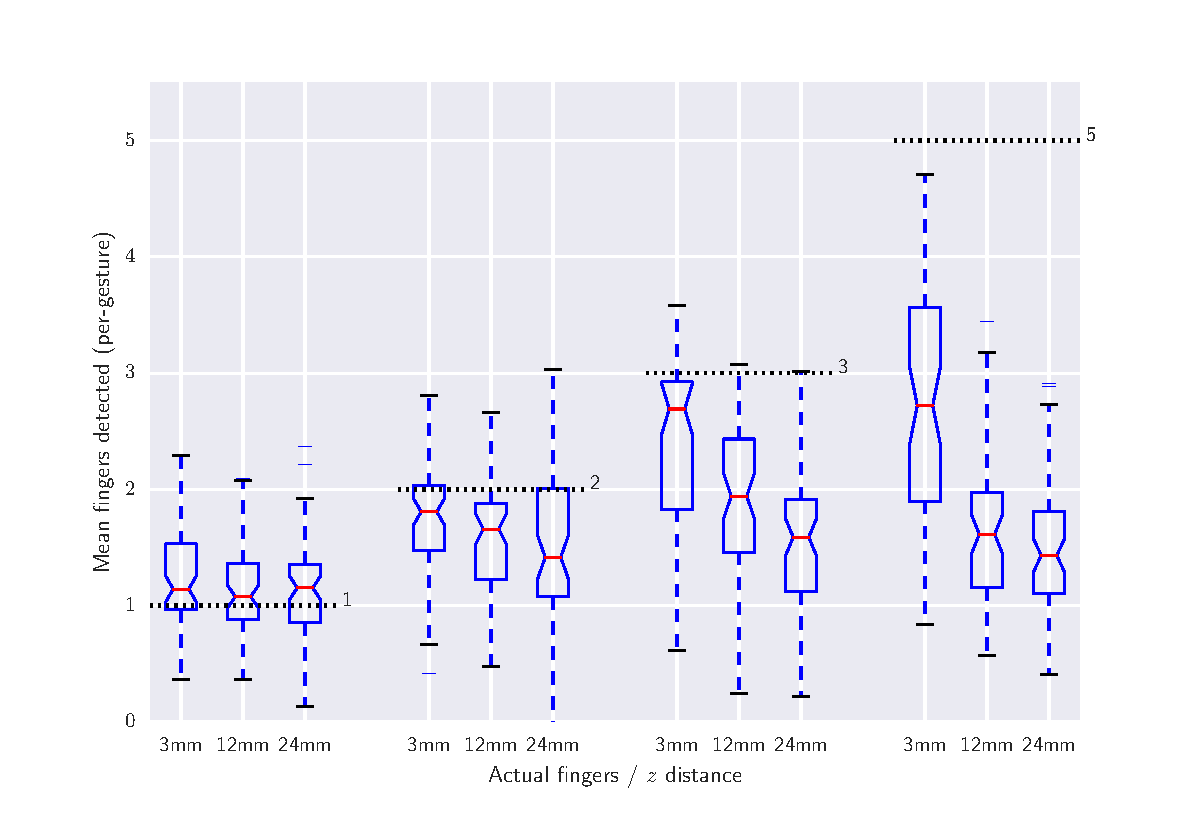
\includegraphics[width=1.0\linewidth]{images/boxplot_finger_distance.pdf}    

%     \caption{Average number of fingers detected by the touch sensor at different heights above the surface, averaged over all gestures. Dashed lines indicate
%     the true number of fingers present. The Box plots include bootstrapped uncertainty notches for the median. It is clear that the device is biased toward 
%     undercounting fingers, particularly at higher $z$ distances.
%     }

%     % use the notation fig:name to cross reference a figure
%     \label{fig:boxplot} 
% \end{figure}


%==================================================================================================================================

% \chapter{Related Work}
% Background will discuss relevant information to understand this project. Related work will discuss other approaches to the topic.

% Maybe mention generative text like code - this cannot be effectively paraphrased.

%==================================================================================================================================
\chapter{Conclusion}    
Summarise the whole project for a lazy reader who didn't read the rest (e.g. a prize-awarding committee).
\section{Guidance}
\begin{itemize}
    \item
        Summarise briefly and fairly.
    \item
        You should be addressing the general problem you introduced in the
        Introduction.        
    \item
        Include summary of concrete results (``the new compiler ran 2x
        faster'')
    \item
        Indicate what future work could be done, but remember: \textbf{you
        won't get credit for things you haven't done}.
\end{itemize}

\section{Limitations}
    % Don't forget to write about how code cannot be word-replaced or paraphrased easily.

\section{Future Work}
\section{Personal Thoughts}

%====== ============================================================================================================================
%
% 
%==================================================================================================================================
%  APPENDICES  

\begin{appendices}

\chapter{Appendices}

Typical inclusions in the appendices are:

\begin{itemize}
\item
  Copies of ethics approvals (required if obtained)
\item
  Copies of questionnaires etc. used to gather data from subjects.
\item
  Extensive tables or figures that are too bulky to fit in the main body of
  the report, particularly ones that are repetitive and summarised in the body.

\item Outline of the source code (e.g. directory structure), or other architecture documentation like class diagrams.

\item User manuals, and any guides to starting/running the software.

\end{itemize}

\textbf{Don't include your source code in the appendices}. It will be
submitted separately.

\end{appendices}

%==================================================================================================================================
%   BIBLIOGRAPHY   

% The bibliography style is abbrvnat
% The bibliography always appears last, after the appendices.

\bibliographystyle{abbrvnat}

\bibliography{l4proj}

\end{document}
